\chapter*{DSPラジオの原理 〜AM編〜}
最近aitendoさんから発売され、個人的に気になっているDSP AM/FMラジオキットの
原理を説明する。一般にラジオは、アンテナで受信した電波を共振回路に入力することで
選局し、それを検波回路に入力し、音声信号を取り出して、アンプで増幅してスピーカーで
音にしている。

これらはアナログ回路であり、例えば共振回路は、コイルとコンデンサーを使ったもので
おそらくコンデンサーの容量を変化させて、共振周波数、すなわち受信する周波数を決定しているし、
検波回路はダイオードの線形性を使って実現されている。
一方でDSPラジオでは、共振回路は同様だが、検波回路はIQ復調と呼ばれる方法が
用いられている。
aitendoさんのDSPラジオでは、AMとFMを聴くことができる。今回はAMの復調原理を説明する。
FMは次号としよう。

前回同様、私の思考の過程を読者が辿れるようにするため、冗長なのは百も承知だが、
数式の過程はできるだけ省かないことにする。


\section*{AM変調とは}
Maxwellが電磁波の存在を理論的に示し、ヘルツによって電磁波の存在が実験的に確認され、
マルコーニよって無線通信の実証が行われた。この時の電波は、まだ変調されておらず
モールス信号のような、電波のON/OFFのパターンで情報を表現するものだった。
この方式では、文字を伝えることはできるのだが、効率が悪く、熟練者でも1分間に
200~300文字程度しか送れず、音声のような情報量の多い通信は不可能である。
そこで、電波をON/OFFでなく、連続的に変化させることで電波に情報を乗せることが
考えられた。この電波に情報を乗せることを変調という。

周波数$f$の電波がアンテナに受信された時、その出力電圧を$V$とすると、
\begin{equation}
V = A\sin(2 \pi f t + \phi) = A\sin(\omega t + \phi)
\end{equation}
と書ける。ここで$A$を振幅、$\omega=2\pi f$を角振動数、$t$は時間、$\phi$を初期位相とする。
この$A$を変化させて信号を乗せるのが、AM (Amplitude Modulation: 振幅変調)である。ちなみに$f$を変化させるのがFM (Frequency Modulation: 周波数変調)、$\phi$を変化さセルのがPM (Phase Modulation: 位相変調)である。

変調によって、信号は電波に乗せられる。信号を乗せる電波のことを搬送波(Carrier)という。この搬送波の周波数を$f_c$、振幅を$C$とすると、搬送波は
\begin{equation}
V_c = C\sin(2 \pi f_c t) = C\sin\omega_c t
\end{equation}
と書ける。
一方、信号波$V_z$は、音声信号が単一の周波数$f_s$のみで構成されているとすると、振幅をSとすると、以下のように書ける。
\begin{equation}
V_s = S\sin(2 \pi f_s t) = S\sin\omega_s t \label{eq:AM_sig}
\end{equation}
\begin{figure}
\scalebox{0.2}{\rotatebox{-90}{\includegraphics{sig.ps}}}
\scalebox{0.2}{\rotatebox{-90}{\includegraphics{carr.ps}}}\\
\scalebox{0.2}{\rotatebox{-90}{\includegraphics{am.ps}}}
\caption{信号波(上段左)、搬送波(上段右)、AM変調波(下段)の例}
\end{figure}

この搬送波$V_c$が、$V_s$にAM変調されると、
\begin{eqnarray}
V_m &=& (V_s + C)\sin\omega_c \label{eq:AM}\\ 
&=&(S\sin\omega_s t + C)\sin\omega_c t \nonumber \\
&=& V_s\sin\omega_s t \sin\omega_c t + C\sin\omega_c \nonumber \\
&=& \frac{V_s}{2}{\sin(\omega_c + \omega_s)t + \sin(\omega_c - \omega_s)t} + C\sin\omega_ct \label{eq:AM_exp}
\end{eqnarray}
となる。ここでは三角関数の公式$\sin\alpha\sin\beta=\frac{1}{2}{\sin(\alpha+\beta)+\sin(\alpha-\beta)}$を用いた。式(\ref{eq:AM_exp})を見ると、AM変調波は、$\omega_s \pm \omega_c$と、$\omega_c$の3つの周波数成分をもっていることがわかる。
話を簡単にするために、信号は$\omega_s$の単一の周波数成分しかもたないことを仮定したが、実際は複数の周波数成分をもっている。よって式(\ref{eq:AM})は、
\begin{eqnarray}
V_m &=&  (\sum_n s_n\sin\omega_n t + C)\sin\omega_c t \nonumber \\
&=& \sum_n a_n\sin\omega_n t \sin\omega_c t + C\sin\omega_c \nonumber \\
&=& \frac{1}{2}\sum_n{a_n\{\sin(\omega_c + \omega_s)t + \sin(\omega_c - \omega_s)t}\} + C\sin\omega_ct \nonumber
\end{eqnarray}
となる。これはシグマが付いているだけで、式(\ref{eq:AM_exp})と同じ形であるので、これ以降、信号波単一の周波数成分からなるものとする。

\section*{IQ復調}
さて、ようやく本題であるDSPラジオの原理を説明しよう。放送局から送信されたAM変調波を式(\ref{eq:AM})で書ける信号をアンテナから受信する。これから搬送波と信号波を分離し、信号波を取り出すことを復調という。つまり式(\ref{eq:AM})から式(\ref{eq:AM_sig})を取り出すことが復調である。

\begin{figure}
\scalebox{0.3}{\includegraphics{blockdiag.eps}}
\caption{DSPラジオIC SI4825-A10 のブロックダイアグラム}
\label{fig:block}
\end{figure}
aitendoさんのDSPラジオキットで使用されているDSPラジオIC Si4825-A10のデータシートにあるブロックダイアグラムを図\ref{fig:block}に示す。アンテナから入力された信号は、ALC(Auto Level Control)回路で増幅率を制御された低ノイズアンプ(LNA)で増幅することで入力レベルを一定にしている。
XTAL1ピンから入力された正弦波をAFC(Automatic Frequency Control)回路で周波数を制御して発信器に入力することで、局部発信器(Local Oscillator)を構成している。局部発信器で作った正弦波を2分割し、一方の位相を90度変化させ、アンテナから入力された信号とDouble Balanced Mixerでそれぞれ混合する。位相を90度変化させた正弦波とアンテナからの入力を混合したものをQ成分、位相を変化させない正弦波と混合したものをI成分と呼ぶ。ミキサーからの出力はLow Pass Filter (LPF)を通りDSPに入力されている。

局部発信器ので作られた正弦波の周波数を$f_L$し、振幅を$A_L$とすると、局部発信器の出力は
\begin{equation}
V_L = A_L \sin(2 \pi f_L t) = A_L \sin\omega_Lt
\end{equation}
となる。ここで$\omega_L = 2\pi f_L$である。Double Balanced Mixerは、二つの入力端子の積が出力する。I成分のMixer出力は、
\begin{eqnarray}
V_I &=& V_mA_L\sin(\omega_Lt + \frac{\pi}{2}) \nonumber\\
&=& V_mA_L\cos\omega_Lt \nonumber\\
&=& (V_s + C)\sin\omega_ct\cos\omega_Lt \nonumber\\
&=& \frac{V_s + C}{2}\{\sin(\omega_c + \omega_L)t + \sin(\omega_c - \omega_L)t \label{eq:AM_I}
\end{eqnarray}
であり、Q成分も同様に
\begin{eqnarray}
V_Q &=& V_mA_L\sin\omega_Lt \nonumber\\
&=& (V_s + C)\sin\omega_ct\sin\omega_Lt \nonumber\\
&=& \frac{V_s + C}{2}\{\cos(\omega_c + \omega_L)t - \cos(\omega_c - \omega_L)t \}\label{eq:AM_Q}
\end{eqnarray}
である。
\begin{figure}
\begin{minipage}{0.5\hsize}
\scalebox{0.2}{\rotatebox{-90}{\includegraphics{i.ps}}}
\caption{I成分}
\end{minipage}
\begin{minipage}{0.5\hsize}
\scalebox{0.2}{\rotatebox{-90}{\includegraphics{q.ps}}}
\caption{Q成分}
\end{minipage}
\end{figure}
Mixerの出力は、LPFで$\omega_c + \omega_L$の成分を除去した後DSPに入力されているので、DSPに入力されるI成分、Q成分は以下の通りである。
\begin{eqnarray}
V_I' &=& \frac{V_s+C}{2}\cos(\omega_c - \omega_L) \label{eq:AM_DSP_I}\\
V_Q' &=& \frac{V_s+C}{2}\sin(\omega_c - \omega_L) \label{eq:AM_DSP_Q}
\end{eqnarray}
DSPでは、式(\ref{eq:AM_DSP_I})と式(\ref{eq:AM_DSP_Q})の二乗の和の平方根、すなわち
\begin{eqnarray}
\sqrt{V_I'^2 + V_Q'^2} &=& \frac{V_s+C}{2}\sqrt{\cos^2(\omega_c - \omega_L)t + \sin^2(\omega_c - \omega_L)t }\\
&=& \frac{V_s+C}{2} 
\end{eqnarray}
を計算する。これで搬送波の周波数成分および局部発信器の周波数成分を除去することができた。
搬送波の振幅である$C$が残っているが、アンテナからの入力は、ALCで増幅率を制御された
低ノイズアンプによって入力レベルが一定なっている。すなわち$C$は一定であるので、DSPで
高域フィルタ(HPF)をかけることで、直流成分$C$を除去することができる。
これが、IQ復調によるAM変調波の復調の原理である。
最後に必要に応じて高調波成分をLPFで除去し、スピーカーで音が出る程度にアンプで復調波を増幅してあげれば、AMラジオのできあがりである。
\begin{figure}
\begin{minipage}{0.5\hsize}
\scalebox{0.2}{\rotatebox{-90}{\includegraphics{demodulate.ps}}}
\end{minipage}
\begin{minipage}{0.5\hsize}
\scalebox{0.2}{\rotatebox{-90}{\includegraphics{out.ps}}}
\end{minipage}
\end{figure}

\lstset{language=R}
\lstinputlisting[caption=シミュレーションのソースコード]{sim.R}
